\documentclass{beamer}

%
% Common preamble for all three parts.
%

\usepackage[spanish]{babel}
\usepackage{amsmath}
\usepackage{color}
\usepackage{minted}
%\setminted{encoding=utf-8}
\usepackage{hyperref}
\usepackage{multicol}
\usepackage{tabularx}
\usepackage{tikz}

\usepackage[utf8]{inputenc}
\usepackage[T1]{fontenc}



% only inline todonotes work
\usepackage{xkeyval}
\usepackage[textsize=small]{todonotes}
\presetkeys{todonotes}{inline}{}

\usetikzlibrary{shapes,arrows,positioning,shadows}

% no nav buttons
\usenavigationsymbolstemplate{}

\newcommand{\bftt}[1]{\textbf{\texttt{#1}}}
\newcommand{\comment}[1]{{\color[HTML]{008080}\textit{\textbf{\texttt{#1}}}}}
\newcommand{\cmd}[1]{{\color[HTML]{008000}\bftt{#1}}}
\newcommand{\bs}{\char`\\}
\newcommand{\cmdbs}[1]{\cmd{\bs#1}}
\newcommand{\lcb}{\char '173}
\newcommand{\rcb}{\char '175}
\newcommand{\cmdbegin}[1]{\cmdbs{begin\lcb}\bftt{#1}\cmd{\rcb}}
\newcommand{\cmdend}[1]{\cmdbs{end\lcb}\bftt{#1}\cmd{\rcb}}

\newcommand{\wllogo}{\textbf{Overleaf}}

% this is where the example source files are loaded from
% do not include a trailing slash
\newcommand{\fileuri}{https://raw.github.com/jdleesmiller/latex-course/master/en}

\newcommand{\wlserver}{https://www.overleaf.com}
\newcommand{\wlnewdoc}[1]{\wlserver/docs?snip\_uri=\fileuri/#1\&splash=none}

\def\tikzname{Ti\emph{k}Z}

% from http://tex.stackexchange.com/questions/5226/keyboard-font-for-latex
\newcommand*\keystroke[1]{%
  \tikz[baseline=(key.base)]
    \node[%
      draw,
      fill=white,
      drop shadow={shadow xshift=0.25ex,shadow yshift=-0.25ex,fill=black,opacity=0.75},
      rectangle,
      rounded corners=2pt,
      inner sep=1pt,
      line width=0.5pt,
      font=\scriptsize\sffamily
    ](key) {#1\strut}
  ;
}
\newcommand{\keystrokebftt}[1]{\keystroke{\bftt{#1}}}

% stolen from minted.dtx
\newenvironment{exampletwoup}
  {\VerbatimEnvironment
   \begin{VerbatimOut}{example.out}}
  {\end{VerbatimOut}
   \setlength{\parindent}{0pt}
   \fbox{\begin{tabular}{l|l}
   \begin{minipage}{0.55\linewidth}
     \inputminted[fontsize=\small,resetmargins]{latex}{example.out}
   \end{minipage} &
   \begin{minipage}{0.35\linewidth}
     \input{example.out}
   \end{minipage}
   \end{tabular}}}

\newenvironment{exampletwouptiny}
  {\VerbatimEnvironment
   \begin{VerbatimOut}{example.out}}
  {\end{VerbatimOut}
   \setlength{\parindent}{0pt}
   \fbox{\begin{tabular}{l|l}
   \begin{minipage}{0.55\linewidth}
     \inputminted[fontsize=\scriptsize,resetmargins]{latex}{example.out}
   \end{minipage} &
   \begin{minipage}{0.35\linewidth}
     \setlength{\parskip}{6pt plus 1pt minus 1pt}%
     \raggedright\scriptsize\input{example.out}
   \end{minipage}
   \end{tabular}}}

\newenvironment{exampletwouptinynoframe}
  {\VerbatimEnvironment
   \begin{VerbatimOut}{example.out}}
  {\end{VerbatimOut}
   \setlength{\parindent}{0pt}
   \begin{tabular}{l|l}
   \begin{minipage}{0.55\linewidth}
     \inputminted[fontsize=\scriptsize,resetmargins]{latex}{example.out}
   \end{minipage} &
   \begin{minipage}{0.35\linewidth}
     \setlength{\parskip}{6pt plus 1pt minus 1pt}%
     \raggedright\scriptsize\input{example.out}
   \end{minipage}
   \end{tabular}}

\title{Una Introducción Interactiva a \LaTeX}
\author{Dr John D. Lees-Miller\\\vspace{.3cm}
  \emph{Traducción: Ing. Luis A. Guanuco}}
\titlegraphic{%
\hspace{1cm}
\includegraphics[width=.2\textwidth]{images/logoCEE}\hfill

\includegraphics[width=.17\textwidth]{images/logoDTO}\hspace{1cm}
}


\subtitle{Parte 2: Documentos Estructurados y Más}

\begin{document}

%%%%%%%%%%%%%%%%%%%%%%%%%%%%%%%%%%%%%%%%%%%%%%%%%%%%%%%%%%%%%%%%%%%%%%%%%%%%%%%
%%%%%%%%%%%%%%%%%%%%%%%%%%%%%%%%%%%%%%%%%%%%%%%%%%%%%%%%%%%%%%%%%%%%%%%%%%%%%%%
%%%%%%%%%%%%%%%%%%%%%%%%%%%%%%%%%%%%%%%%%%%%%%%%%%%%%%%%%%%%%%%%%%%%%%%%%%%%%%%
\begin{frame}
\titlepage
\end{frame}

%%%%%%%%%%%%%%%%%%%%%%%%%%%%%%%%%%%%%%%%%%%%%%%%%%%%%%%%%%%%%%%%%%%%%%%%%%%%%%%
%%%%%%%%%%%%%%%%%%%%%%%%%%%%%%%%%%%%%%%%%%%%%%%%%%%%%%%%%%%%%%%%%%%%%%%%%%%%%%%
%%%%%%%%%%%%%%%%%%%%%%%%%%%%%%%%%%%%%%%%%%%%%%%%%%%%%%%%%%%%%%%%%%%%%%%%%%%%%%%
\section{Documentos Estructurados}

%%%%%%%%%%%%%%%%%%%%%%%%%%%%%%%%%%%%%%%%%%%%%%%%%%%%%%%%%%%%%%%%%%%%%%%%%%%%%%%
%%%%%%%%%%%%%%%%%%%%%%%%%%%%%%%%%%%%%%%%%%%%%%%%%%%%%%%%%%%%%%%%%%%%%%%%%%%%%%% 
%%%%%%%%%%%%%%%%%%%%%%%%%%%%%%%%%%%%%%%%%%%%%%%%%%%%%%%%%%%%%%%%%%%%%%%%%%%%%%% 
\begin{frame}{Outline}
  \begin{multicols}{2}
    \tableofcontents[currentsection]
  \end{multicols}
\end{frame}

%%%%%%%%%%%%%%%%%%%%%%%%%%%%%%%%%%%%%%%%%%%%%%%%%%%%%%%%%%%%%%%%%%%%%%%%%%%%%%%
%%%%%%%%%%%%%%%%%%%%%%%%%%%%%%%%%%%%%%%%%%%%%%%%%%%%%%%%%%%%%%%%%%%%%%%%%%%%%%%
%%%%%%%%%%%%%%%%%%%%%%%%%%%%%%%%%%%%%%%%%%%%%%%%%%%%%%%%%%%%%%%%%%%%%%%%%%%%%%%
\begin{frame}{\insertsection}
  \begin{itemize}
  \item En la Parte 1, aprendimos acerca de los comandos y entornos
    para la tipografía de texto y contenido matemático.
  \item Ahora, vamos a conocer acerca de los comandos y entornos para
    generar documentos estructurados.
  \item Puede probar los nuevos comandos en Overleaf:
  \end{itemize}
  \vskip 2em
  \begin{center}
    \fbox{\href{\wlnewdoc{basics.tex}}{%
        Click aquí para abrir el documento de ejemplo en \wllogo{}}}
    \\[1ex]\scriptsize{}
    Para un mejor resultado, use
      \href{http://www.google.com/chrome}{Google Chrome} o una versión
      actualizada de \href{http://www.mozilla.org/en-US/firefox/new/}{FireFox}.
  \end{center}
  \vskip 2ex
  \begin{itemize}
  \item Vamos a comenzar!
  \end{itemize}
\end{frame}

%%%%%%%%%%%%%%%%%%%%%%%%%%%%%%%%%%%%%%%%%%%%%%%%%%%%%%%%%%%%%%%%%%%%%%%%%%%%%%%
%%%%%%%%%%%%%%%%%%%%%%%%%%%%%%%%%%%%%%%%%%%%%%%%%%%%%%%%%%%%%%%%%%%%%%%%%%%%%%%
%%%%%%%%%%%%%%%%%%%%%%%%%%%%%%%%%%%%%%%%%%%%%%%%%%%%%%%%%%%%%%%%%%%%%%%%%%%%%%% 
\subsection{Título y Resumen}
\begin{frame}[fragile]{\insertsubsection}
  \begin{itemize}{\small
    \item Le decimos a \LaTeX{} el \cmdbs{title} y nombre del
      \cmdbs{author} en el preámbulo.
    \item Luego utilizamos el comando \cmdbs{maketitle} en el
      documento para  visualizarlos en la salida.
    \item Utilice el entorno \bftt{abstract} para crear un resumen.
    }\end{itemize}
  \begin{minipage}{0.55\linewidth}
    \inputminted[fontsize=\scriptsize,frame=single,resetmargins]{latex}%
    {structure-title.tex}
  \end{minipage}
  \begin{minipage}{0.35\linewidth}
    \includegraphics[width=\textwidth,clip,trim=2.2in 7in 2.2in 2in]{structure-title.pdf}
  \end{minipage}
\end{frame}

%%%%%%%%%%%%%%%%%%%%%%%%%%%%%%%%%%%%%%%%%%%%%%%%%%%%%%%%%%%%%%%%%%%%%%%%%%%%%%% 
%%%%%%%%%%%%%%%%%%%%%%%%%%%%%%%%%%%%%%%%%%%%%%%%%%%%%%%%%%%%%%%%%%%%%%%%%%%%%%%
%%%%%%%%%%%%%%%%%%%%%%%%%%%%%%%%%%%%%%%%%%%%%%%%%%%%%%%%%%%%%%%%%%%%%%%%%%%%%%%
\subsection{Secciones}
\begin{frame}{\insertsubsection}
  \begin{itemize}{\small
    \item Solo utilice \cmdbs{section} y \cmdbs{subsection}.
    \item ¿Pueden adivinar qué hacen los comandos \cmdbs{section*} y \cmdbs{subsection*}?
    }\end{itemize}
  \begin{minipage}{0.55\linewidth}
    \inputminted[fontsize=\scriptsize,frame=single,resetmargins]{latex}%
    {structure-sections.tex}
  \end{minipage}
  \begin{minipage}{0.35\linewidth}
    \includegraphics[width=\textwidth,clip,trim=1.5in 6in 4in 1in]{structure-sections.pdf}
  \end{minipage}
\end{frame}

%%%%%%%%%%%%%%%%%%%%%%%%%%%%%%%%%%%%%%%%%%%%%%%%%%%%%%%%%%%%%%%%%%%%%%%%%%%%%%%
%%%%%%%%%%%%%%%%%%%%%%%%%%%%%%%%%%%%%%%%%%%%%%%%%%%%%%%%%%%%%%%%%%%%%%%%%%%%%%%
%%%%%%%%%%%%%%%%%%%%%%%%%%%%%%%%%%%%%%%%%%%%%%%%%%%%%%%%%%%%%%%%%%%%%%%%%%%%%%%
\subsection{Etiquetas y Referencias Cruzadas}
\begin{frame}[fragile]{\insertsubsection}
  \begin{itemize}{\small
    \item Utilice \cmdbs{label} y \cmdbs{ref} para la numeración automática.
    \item El paquete \bftt{amsmath} proporciona \cmdbs{eqref} para
      las referencias de ecuaciones.
    }\end{itemize}
  \begin{minipage}{0.55\linewidth}
    \inputminted[fontsize=\scriptsize,frame=single,resetmargins]{latex}%
    {structure-crossref.tex}
  \end{minipage}
  \begin{minipage}{0.35\linewidth}
    \includegraphics[width=\textwidth,clip,trim=1.8in 6in 1.6in 1in]{structure-crossref.pdf}
  \end{minipage}
\end{frame}

%%%%%%%%%%%%%%%%%%%%%%%%%%%%%%%%%%%%%%%%%%%%%%%%%%%%%%%%%%%%%%%%%%%%%%%%%%%%%%%
%%%%%%%%%%%%%%%%%%%%%%%%%%%%%%%%%%%%%%%%%%%%%%%%%%%%%%%%%%%%%%%%%%%%%%%%%%%%%%%
%%%%%%%%%%%%%%%%%%%%%%%%%%%%%%%%%%%%%%%%%%%%%%%%%%%%%%%%%%%%%%%%%%%%%%%%%%%%%%%
\subsection{Ejercitación}
\begin{frame}[fragile]{Ejercicio de Documentos Estructurados}
  
  \begin{block}{Escriba este pequeño artículo en \LaTeX:
      \footnote{Desde \url{http://pdos.csail.mit.edu/scigen/}, un
        generador aleatorio de artículos.}}
    \begin{center}
      \fbox{\href{\fileuri/structure-exercise-solution.pdf}{%
          Click para abrir el artículo}}
    \end{center}
    Haga su versión del artículo mirando el artículo original. Utilice
     \cmdbs{ref} y \cmdbs{eqref} para evitar escribir explícitamente
     la sección y el número de ecuación dentro del texto.
  \end{block}
  \vskip 2ex
  \begin{center}
    \fbox{\href{\wlnewdoc{structure-exercise.tex}}{%
        Click para abrir el ejercicio en  \wllogo{}}}
  \end{center}
  
  \begin{itemize}
  \item Una vez que lo haya probado,
    \fbox{\href{\wlnewdoc{structure-exercise-solution.tex}}{%
        click aquí para ver la solución}}.
  \end{itemize}
\end{frame}

%%%%%%%%%%%%%%%%%%%%%%%%%%%%%%%%%%%%%%%%%%%%%%%%%%%%%%%%%%%%%%%%%%%%%%%%%%%%%%%
%%%%%%%%%%%%%%%%%%%%%%%%%%%%%%%%%%%%%%%%%%%%%%%%%%%%%%%%%%%%%%%%%%%%%%%%%%%%%%%
%%%%%%%%%%%%%%%%%%%%%%%%%%%%%%%%%%%%%%%%%%%%%%%%%%%%%%%%%%%%%%%%%%%%%%%%%%%%%%%
\section{Figuras y Tablas}

%%%%%%%%%%%%%%%%%%%%%%%%%%%%%%%%%%%%%%%%%%%%%%%%%%%%%%%%%%%%%%%%%%%%%%%%%%%%%%%
%%%%%%%%%%%%%%%%%%%%%%%%%%%%%%%%%%%%%%%%%%%%%%%%%%%%%%%%%%%%%%%%%%%%%%%%%%%%%%%
%%%%%%%%%%%%%%%%%%%%%%%%%%%%%%%%%%%%%%%%%%%%%%%%%%%%%%%%%%%%%%%%%%%%%%%%%%%%%%%
\begin{frame}{Outline}
  \begin{multicols}{2}
    \tableofcontents[currentsection]
  \end{multicols}
\end{frame}

%%%%%%%%%%%%%%%%%%%%%%%%%%%%%%%%%%%%%%%%%%%%%%%%%%%%%%%%%%%%%%%%%%%%%%%%%%%%%%%
%%%%%%%%%%%%%%%%%%%%%%%%%%%%%%%%%%%%%%%%%%%%%%%%%%%%%%%%%%%%%%%%%%%%%%%%%%%%%%%
%%%%%%%%%%%%%%%%%%%%%%%%%%%%%%%%%%%%%%%%%%%%%%%%%%%%%%%%%%%%%%%%%%%%%%%%%%%%%%%
\subsection{Gráficos}
\begin{frame}[fragile]{\insertsubsection}
  \begin{itemize}
  \item Requiere del paquete \bftt{graphicx}, que proporciona el
    comando \cmdbs{includegraphics}.
  \item Los formatos gráficos soportados incluyen JPEG, PNG y PDF.
  \end{itemize}
  \begin{exampletwouptiny}
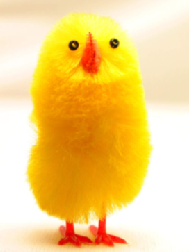
\includegraphics[
width=0.5\textwidth]{big_chick}

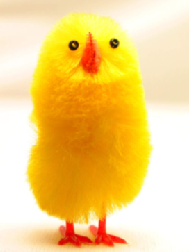
\includegraphics[
width=0.3\textwidth,
angle=270]{big_chick}
  \end{exampletwouptiny}
  
  \tiny{Imagen desde \url{http://www.andy-roberts.net/writing/latex/importing_images}}
\end{frame}

%%%%%%%%%%%%%%%%%%%%%%%%%%%%%%%%%%%%%%%%%%%%%%%%%%%%%%%%%%%%%%%%%%%%%%%%%%%%%%% 
%%%%%%%%%%%%%%%%%%%%%%%%%%%%%%%%%%%%%%%%%%%%%%%%%%%%%%%%%%%%%%%%%%%%%%%%%%%%%%% 
%%%%%%%%%%%%%%%%%%%%%%%%%%%%%%%%%%%%%%%%%%%%%%%%%%%%%%%%%%%%%%%%%%%%%%%%%%%%%%%
\begin{frame}[fragile]{Intermedio: Argumentos Opcionales}
  \begin{itemize}
  \item Utilizamos corchetes  \keystrokebftt{[} \keystrokebftt{]} para
    los argumentos opcionales, en lugar de las llaves \keystrokebftt{\{} \keystrokebftt{\}}.
  \item \cmdbs{includegraphics} acepta argumentos opcionales que
    permiten transformar la imagen cuando se incluya. Por ejemplo,
    \bftt{width=0.3\cmdbs{textwidth}}  hace que la imagen ocupe el
    30\% del ancho total asignado para el texto (\cmdbs{textwidth}).
  \item \cmdbs{documentclass} también acepta argumentos
    opcionales. Por ejemplo:
    \mint{latex}|\documentclass[12pt,twocolumn]{article}|
    \vskip 3ex
    hace al texto más grande (12pt) y lo coloca en dos columnas.
  \item ¿Dónde encontramos información sobre estas cosas? Vea las
    diapositivas hasta el final para obtener enlaces a más información.
  \end{itemize}
\end{frame}

%%%%%%%%%%%%%%%%%%%%%%%%%%%%%%%%%%%%%%%%%%%%%%%%%%%%%%%%%%%%%%%%%%%%%%%%%%%%%%%
%%%%%%%%%%%%%%%%%%%%%%%%%%%%%%%%%%%%%%%%%%%%%%%%%%%%%%%%%%%%%%%%%%%%%%%%%%%%%%%
%%%%%%%%%%%%%%%%%%%%%%%%%%%%%%%%%%%%%%%%%%%%%%%%%%%%%%%%%%%%%%%%%%%%%%%%%%%%%%%
\subsection[fragile]{Flotantes}
\begin{frame}{\insertsubsection}
  \begin{itemize}
  \item Permita a \LaTeX decidir dónde se ubicará la figura (ésta
    puede ``flotar'').
  \item Puede también darle a la figura un título, que puede ser
    referenciado con \cmdbs{ref}.
  \end{itemize}
  \begin{minipage}{0.55\linewidth}
    \inputminted[fontsize=\scriptsize,frame=single,resetmargins]{latex}%
    {media-graphics.tex}
  \end{minipage}
  \begin{minipage}{0.35\linewidth}
    \includegraphics[width=\textwidth,clip,trim=2in 5in 3in 1in]{media-graphics.pdf}
  \end{minipage}
\end{frame}

%%%%%%%%%%%%%%%%%%%%%%%%%%%%%%%%%%%%%%%%%%%%%%%%%%%%%%%%%%%%%%%%%%%%%%%%%%%%%%%
%%%%%%%%%%%%%%%%%%%%%%%%%%%%%%%%%%%%%%%%%%%%%%%%%%%%%%%%%%%%%%%%%%%%%%%%%%%%%%%
%%%%%%%%%%%%%%%%%%%%%%%%%%%%%%%%%%%%%%%%%%%%%%%%%%%%%%%%%%%%%%%%%%%%%%%%%%%%%%%
\subsection{Tablas}
\begin{frame}[fragile]{\insertsubsection}
  \begin{itemize}
  \item Las tablas en \LaTeX{} requieren un tiempo para acostumbrarse.
%  \item Utilice el entorno \bftt{tabular} desde el paquete
%\bftt{tabularx}.
  \item El argumento especifica la alineación de las columnas ---
\textbf{l}eft, \textbf{r}ight, \textbf{r}ight.
    \begin{exampletwouptiny}
\begin{tabular}{lrr}
  Art.   & Cant. & Uni. \$ \\
  DVD    & 1     & 19.99   \\
  Sonido & 2     & 39.99   \\
  Cable  & 3     & 1.99    \\
\end{tabular}
    \end{exampletwouptiny}
  \item También se especifican las líneas verticales; utilice el
comando \cmdbs{hline} para las líneas horizontales.
    \begin{exampletwouptiny}
\begin{tabular}{|l|r|r|}    \hline
  Art.   & Cant. & Uni.\$ \\\hline
  DVD    & 1     & 19.99  \\
  Sonido & 2     & 39.99  \\
  Cable  & 3     & 1.99   \\\hline
\end{tabular}
    \end{exampletwouptiny}
  \item Utilice un ampersand \keystrokebftt{\&} para separarlas
columnas y una doble barra invertida
\keystrokebftt{\bs}\keystrokebftt{\bs} para comenzar una nueva
fila(como en el entorno \bftt{align*} visto en la Parte 1).
  \end{itemize}
\end{frame}

%%%%%%%%%%%%%%%%%%%%%%%%%%%%%%%%%%%%%%%%%%%%%%%%%%%%%%%%%%%%%%%%%%%%%%%%%%%%%%% 
%%%%%%%%%%%%%%%%%%%%%%%%%%%%%%%%%%%%%%%%%%%%%%%%%%%%%%%%%%%%%%%%%%%%%%%%%%%%%%% 
%%%%%%%%%%%%%%%%%%%%%%%%%%%%%%%%%%%%%%%%%%%%%%%%%%%%%%%%%%%%%%%%%%%%%%%%%%%%%%%
\addtocontents{toc}{\newpage}
\section{Bibliografías}

%%%%%%%%%%%%%%%%%%%%%%%%%%%%%%%%%%%%%%%%%%%%%%%%%%%%%%%%%%%%%%%%%%%%%%%%%%%%%%%
%%%%%%%%%%%%%%%%%%%%%%%%%%%%%%%%%%%%%%%%%%%%%%%%%%%%%%%%%%%%%%%%%%%%%%%%%%%%%%%
%%%%%%%%%%%%%%%%%%%%%%%%%%%%%%%%%%%%%%%%%%%%%%%%%%%%%%%%%%%%%%%%%%%%%%%%%%%%%%%
\begin{frame}{Outline}
  \begin{multicols}{2}
    \tableofcontents[currentsection]
  \end{multicols}
\end{frame}

%%%%%%%%%%%%%%%%%%%%%%%%%%%%%%%%%%%%%%%%%%%%%%%%%%%%%%%%%%%%%%%%%%%%%%%%%%%%%%%
%%%%%%%%%%%%%%%%%%%%%%%%%%%%%%%%%%%%%%%%%%%%%%%%%%%%%%%%%%%%%%%%%%%%%%%%%%%%%%%
%%%%%%%%%%%%%%%%%%%%%%%%%%%%%%%%%%%%%%%%%%%%%%%%%%%%%%%%%%%%%%%%%%%%%%%%%%%%%%%
\subsection{bib\TeX}
\begin{frame}[fragile]{\insertsubsection{} 1}
  \begin{itemize}
  \item Colocar las referencias en un archivo \bftt{.bib} en el
    formato de base de datos  `bibtex':
    \inputminted[fontsize=\scriptsize,frame=single]{latex}{bib-example.bib}
  \item La mayoría de los gestores de referencias pueden exportar al
    formato bibtex.
  \end{itemize}
\end{frame}

%%%%%%%%%%%%%%%%%%%%%%%%%%%%%%%%%%%%%%%%%%%%%%%%%%%%%%%%%%%%%%%%%%%%%%%%%%%%%%% 
%%%%%%%%%%%%%%%%%%%%%%%%%%%%%%%%%%%%%%%%%%%%%%%%%%%%%%%%%%%%%%%%%%%%%%%%%%%%%%% 
%%%%%%%%%%%%%%%%%%%%%%%%%%%%%%%%%%%%%%%%%%%%%%%%%%%%%%%%%%%%%%%%%%%%%%%%%%%%%%% 
\begin{frame}[fragile]{\insertsubsection{} 2}
  \begin{itemize}
  \item Cada entrada en el archivo  \bftt{.bib} tiene una \emph{clave}
    que puede usar para ser referenciado en el documento. Por ejemplo,
    \bftt{Jacobson1999Towards} es la clave para este artículo:
    \begin{minted}[fontsize=\small,frame=single]{latex}
@Article{Jacobson1999Towards,
  author = {Van Jacobson},
  ...
}
    \end{minted}
  \item Es recomendable utilizar una clave basada en el nombre, año y
    título del artículo.
  \item \LaTeX{} puede formatear automáticamente sus citas en el texto
    y generar una lista de referencias; basados en estilos estándares,
    y hasta se pueden diseñar sus propios estilos.
  \end{itemize}
\end{frame}

%%%%%%%%%%%%%%%%%%%%%%%%%%%%%%%%%%%%%%%%%%%%%%%%%%%%%%%%%%%%%%%%%%%%%%%%%%%%%%% 
%%%%%%%%%%%%%%%%%%%%%%%%%%%%%%%%%%%%%%%%%%%%%%%%%%%%%%%%%%%%%%%%%%%%%%%%%%%%%%%
%%%%%%%%%%%%%%%%%%%%%%%%%%%%%%%%%%%%%%%%%%%%%%%%%%%%%%%%%%%%%%%%%%%%%%%%%%%%%%%
\begin{frame}[fragile]{\insertsubsection{} 3}
  \begin{itemize}
  \item Utilice el paquete \bftt{natbib} \footnote{Hay un nuevo
      paquete con más características llamado \bftt{biblatex} pero la
      mayoría de las plantillas para artículos todavía utiliza
      \bftt{natbib}.} con \cmdbs{citet} y \cmdbs{citep}.
  \item Las referencias Bibliográficas van al final del texto con el
    comando \cmdbs{bibliography}, y luego se especifica el estilo con
    \cmdbs{bibliographystyle}.
  \end{itemize}
  \begin{minipage}{0.55\linewidth}
    \inputminted[fontsize=\scriptsize,frame=single,resetmargins]{latex}%
    {bib-example.tex}
  \end{minipage}
  \begin{minipage}{0.35\linewidth}
    \includegraphics[width=\textwidth,clip,trim=1.8in 5in 1.8in 1in]{bib-example.pdf}
  \end{minipage}
\end{frame}

%%%%%%%%%%%%%%%%%%%%%%%%%%%%%%%%%%%%%%%%%%%%%%%%%%%%%%%%%%%%%%%%%%%%%%%%%%%%%%% 
%%%%%%%%%%%%%%%%%%%%%%%%%%%%%%%%%%%%%%%%%%%%%%%%%%%%%%%%%%%%%%%%%%%%%%%%%%%%%%%
%%%%%%%%%%%%%%%%%%%%%%%%%%%%%%%%%%%%%%%%%%%%%%%%%%%%%%%%%%%%%%%%%%%%%%%%%%%%%%%
\subsection{Ejercitación}
\begin{frame}[fragile]{Ejercicio: Coloque Todo Junto}
  
  Agregue una imagen y una bibliografía al artículo desde el ejercicio prvio.
  
  \begin{enumerate}
  \item Descargue estos archivos de ejemplos a su computadora.

    \begin{center}
      \fbox{\href{\fileuri/big_chick.png?dl=1}{Click aquí para
          descargar imagen}}
      
      \fbox{\href{\fileuri/bib-exercise.bib?dl=1}{Click aquí para
          descargar el archivo bib}}
    \end{center}
    
  \item Súbalos a  Overleaf (Utilice el menú ``project'').
    
  \end{enumerate}
\end{frame}

%%%%%%%%%%%%%%%%%%%%%%%%%%%%%%%%%%%%%%%%%%%%%%%%%%%%%%%%%%%%%%%%%%%%%%%%%%%%%%% 
%%%%%%%%%%%%%%%%%%%%%%%%%%%%%%%%%%%%%%%%%%%%%%%%%%%%%%%%%%%%%%%%%%%%%%%%%%%%%%%
%%%%%%%%%%%%%%%%%%%%%%%%%%%%%%%%%%%%%%%%%%%%%%%%%%%%%%%%%%%%%%%%%%%%%%%%%%%%%%% 
\section{¿Qué Sigue?}

%%%%%%%%%%%%%%%%%%%%%%%%%%%%%%%%%%%%%%%%%%%%%%%%%%%%%%%%%%%%%%%%%%%%%%%%%%%%%%%
%%%%%%%%%%%%%%%%%%%%%%%%%%%%%%%%%%%%%%%%%%%%%%%%%%%%%%%%%%%%%%%%%%%%%%%%%%%%%%%
%%%%%%%%%%%%%%%%%%%%%%%%%%%%%%%%%%%%%%%%%%%%%%%%%%%%%%%%%%%%%%%%%%%%%%%%%%%%%%%
\begin{frame}{Outline}
  \begin{multicols}{2}
    \tableofcontents[currentsection]
  \end{multicols}
\end{frame}

%%%%%%%%%%%%%%%%%%%%%%%%%%%%%%%%%%%%%%%%%%%%%%%%%%%%%%%%%%%%%%%%%%%%%%%%%%%%%%% 
%%%%%%%%%%%%%%%%%%%%%%%%%%%%%%%%%%%%%%%%%%%%%%%%%%%%%%%%%%%%%%%%%%%%%%%%%%%%%%%
%%%%%%%%%%%%%%%%%%%%%%%%%%%%%%%%%%%%%%%%%%%%%%%%%%%%%%%%%%%%%%%%%%%%%%%%%%%%%%%
\subsection{Cosas Más Esmeradas}
\begin{frame}[fragile]{\insertsubsection}
  \begin{itemize}
  \item Agregue el comando  \cmdbs{tableofcontents} para generar una
    tabla de contenidos.
    
  \item Cambie la clase de documento (\cmdbs{documentclass}) a 
    \mint{latex}!\documentclass{scrartcl}! o 
    \mint{latex}!\documentclass[12pt]{IEEEtran}!
    
  \item Defina su propio comando para una ecuación compleja:
    \begin{exampletwouptiny}
      \newcommand{\rperf}{%
  \rho_{\text{perf}}}
$$
\rperf = {\bf c}'{\bf X} + \varepsilon
$$
    \end{exampletwouptiny}
  \end{itemize}
\end{frame}

%%%%%%%%%%%%%%%%%%%%%%%%%%%%%%%%%%%%%%%%%%%%%%%%%%%%%%%%%%%%%%%%%%%%%%%%%%%%%%% 
%%%%%%%%%%%%%%%%%%%%%%%%%%%%%%%%%%%%%%%%%%%%%%%%%%%%%%%%%%%%%%%%%%%%%%%%%%%%%%% 
%%%%%%%%%%%%%%%%%%%%%%%%%%%%%%%%%%%%%%%%%%%%%%%%%%%%%%%%%%%%%%%%%%%%%%%%%%%%%%% 
\subsection{Otros Paquetes Interesantes}
\begin{frame}{\insertsubsection}
  \begin{itemize}
  \item \bftt{beamer}: para presentaciones (igual que éste!)
  \item \bftt{todonotes}: comentarios y manejo de ``TODO''(para hacer)
  \item \bftt{tikz}: hacer increíbles gráficos
  \item \bftt{pgfplots}: crear gráficos en \LaTeX
  \item \bftt{listings}: impresora de código fuente para \LaTeX
  \item \bftt{spreadtab}: crear hojas de cálculos en \LaTeX
  \item \bftt{gchords}, \bftt{guitar}: Acordes de guitarra y tablatura
  \item \bftt{cwpuzzle}: crucigramas
  \end{itemize}
  Ver \url{https://www.overleaf.com/latex/examples} y \url{http://texample.net}
  para obtener ejemplos de la mayoría de estos paquetes.
\end{frame}

%%%%%%%%%%%%%%%%%%%%%%%%%%%%%%%%%%%%%%%%%%%%%%%%%%%%%%%%%%%%%%%%%%%%%%%%%%%%%%% 
%%%%%%%%%%%%%%%%%%%%%%%%%%%%%%%%%%%%%%%%%%%%%%%%%%%%%%%%%%%%%%%%%%%%%%%%%%%%%%% 
%%%%%%%%%%%%%%%%%%%%%%%%%%%%%%%%%%%%%%%%%%%%%%%%%%%%%%%%%%%%%%%%%%%%%%%%%%%%%%% 
\subsection{Instalación de  \LaTeX{}}
\begin{frame}{\insertsubsection}
  \begin{itemize}
  \item Para ejecutar \LaTeX{} sobre su computadora, deberá utilizar
    una \emph{distribución}. Una distribución incluye un
    programa \bftt{latex} y (típicamente) varios miles de paquetes.
    \begin{itemize}
    \item sobre Windows: \href{http://miktex.org/}{Mik\TeX} o \href{http://tug.org/texlive/}{\TeX Live}
    \item Sobre GNU/Linux: \href{http://tug.org/texlive/}{\TeX Live}
    \item Sobre Mac: \href{http://tug.org/mactex/}{Mac\TeX}
    \end{itemize}
  \item También querrá un editor de texto con sporte para
\LaTeX{}. Vea
\url{http://en.wikipedia.org/wiki/Comparison_of_TeX_editors} para una
lista de muchas opciones.
  \item También tiene que saber más acerca de cómo  \bftt{latex}, y sus
    herramientas relacionadas, trabajan --- consulte las fuentes de la
    siguiente diapositiva. 
  \end{itemize}
\end{frame}

%%%%%%%%%%%%%%%%%%%%%%%%%%%%%%%%%%%%%%%%%%%%%%%%%%%%%%%%%%%%%%%%%%%%%%%%%%%%%%% 
%%%%%%%%%%%%%%%%%%%%%%%%%%%%%%%%%%%%%%%%%%%%%%%%%%%%%%%%%%%%%%%%%%%%%%%%%%%%%%%
%%%%%%%%%%%%%%%%%%%%%%%%%%%%%%%%%%%%%%%%%%%%%%%%%%%%%%%%%%%%%%%%%%%%%%%%%%%%%%%
\subsection{Recursos en Línea}
\begin{frame}{\insertsubsection}
  \begin{itemize}
  \item \href{http://en.wikibooks.org/wiki/LaTeX}{La WikiBook de
      \LaTeX{}} --- excelente tutoriales y materiales de referencia.
  \item \href{http://tex.stackexchange.com/}{\TeX{} Stack Exchange} ---
    haga sus consultas y obtenga excelentes respuestas con una rapidez
    increíble.
  \item \href{http://www.latex-community.org/}{Comunidad \LaTeX{}} ---
    un gran foro en línea
  \item \href{http://ctan.org/}{Comprehensive \TeX{} Archive Network (CTAN)} ---
    más de cuatro mil paquetes, y sus respectivas documentaciones.
  \item Sí utiliza Google seguramente llegará  a uno de los anteriores sitios.
  \end{itemize}
\end{frame}

%%%%%%%%%%%%%%%%%%%%%%%%%%%%%%%%%%%%%%%%%%%%%%%%%%%%%%%%%%%%%%%%%%%%%%%%%%%%%%% 
%%%%%%%%%%%%%%%%%%%%%%%%%%%%%%%%%%%%%%%%%%%%%%%%%%%%%%%%%%%%%%%%%%%%%%%%%%%%%%%
%%%%%%%%%%%%%%%%%%%%%%%%%%%%%%%%%%%%%%%%%%%%%%%%%%%%%%%%%%%%%%%%%%%%%%%%%%%%%%%
\begin{frame}
  \begin{center}
    Gracias!
  \end{center}
\end{frame}

\end{document}

% -- latex understands words, sentences and paragraphs

Words are separated by one or more spaces.  Paragraphs are separated by
one or more blank lines.  The output is not affected by adding extra
spaces or extra blank lines to the input file.

Double quotes are typed like this: ``quoted text''.
Single quotes are typed like this: `single-quoted text'.

Emphasized text is typed like this: \emph{this is emphasized}.
Bold       text is typed like this: \textbf{this is bold}.

-- Adding structure to your document

\section{Hello}

\subsection{World}

\subsection{Foo}

\subsubsection*{Stuff} % star form

\subsubsection*{Results}

-- Labels and cross-references

\label{sec:intro}
\label{sec:method}
\ref{sec:method}

--> maybe introduce the prettyref package here.

-- Mathematics

Inline mathematics: $x + y < 7$.

'Displayed' mathematics:
\begin{equation}
\end{equation}

\begin{equation*}
\end{equation*}

\begin{align}
\end{align}

-- Figures

- Need the graphicx package.

- here we can start introducing options

\includegraphics[width=\textwidth]{}

- where do you find out about these options? --> link to the Wikibook

-- Floating Figures

\begin{figure}
\includegraphics{...}
\caption{\label{}Here is a caption.}
\end{figure}

-- Tables

- not the nicest part of LaTeX

\usepackage{tabularx}

\begin{tabular}{llr}
Item & Quantity & Price (\$) & Amount
Widget & 1 &
\end{tabular}

Bonus points: check out the fp package and the spreadtab package.

-- Document Classes

a .cls file

article

some journal templates come with one

-- Bibliographies



-- For Typesetting Geeks

- dashes: -, --, ---

- ellipsis.

- controlling spaces: ~, \ , \,, \@

- spacing after periods (et al., etc.)

- Nested quotation marks: ``\,`
\vskip 2ex
\item Use the \emph{star form} to display an equation without a number.
\begin{exampletwouptiny}
\begin{equation*}
F(x) = \int_{a}^{x}{f(t) dt}
\end{equation*}
\end{exampletwouptiny}

\begin{itemize}
\item \bftt{equation} and \bftt{equation*} are called \emph{environments}.
\begin{itemize}
  \item The \cmdbs{begin} and \cmdbs{end} commands define the environment.
  \item The \cmd{\$} also starts and ends an environment.
  \item Some commands are defined only within certain environments.
  \item Some commands behave differently in different environments.
\end{itemize}
\end{itemize}
\end{block}
\begin{center}
\fbox{\href{http://ctan.org/}{The Comprehensive \TeX Archive Network (CTAN)}}
\end{center}

%%%%%%%%%%%%%%%%%%%%%%%%%%%%%%%%%%%%%%%%%%%%%%%%%%%%%%%%%%%%%%%%%%%%%%%%%%%%%%%
%%%%%%%%%%%%%%%%%%%%%%%%%%%%%%%%%%%%%%%%%%%%%%%%%%%%%%%%%%%%%%%%%%%%%%%%%%%%%%%
%%%%%%%%%%%%%%%%%%%%%%%%%%%%%%%%%%%%%%%%%%%%%%%%%%%%%%%%%%%%%%%%%%%%%%%%%%%%%%%
\subsection{Typography tweaks}
\begin{frame}{\insertsubsection}
\begin{tabular}{lll}
& character name & used mainly for \ldots \\\hline
\bftt{\bs} & backslash                 & commands, tables \\
\bftt{\{}  & open brace                & commands \\
\bftt{\}}  & close brace               & commands \\
\bftt{\%}  & percent sign              & comments \\
\bftt{\#}  & hash (pound / sharp) sign & custom commands \\
\bftt{\$}  & dollar sign               & equations \\
\bftt{\_}  & underscore                & equations (subscripts) \\
\bftt{\^}  & caret                     & equations (superscripts) \\
\bftt{\&}  & ampersand                 & tables \\
\bftt{\~}  & tilde                     & spacing \\
\end{tabular}
\end{frame}

%\item We've used several environments:
%\vskip 1ex
%{\scriptsize
%\begin{tabular}{ll}
%\cmdbs{begin}\bftt{\{document\}}\ldots\cmdbs{end}\bftt{\{document\}} &
%  document environment \\
%\cmdbs{begin}\bftt{\{itemize\}}\ldots\cmdbs{end}\bftt{\{itemize\}} &
%  itemized list environment \\
%\bftt{\$\ldots\$}     & \emph{in-text} math environment \\
%\bftt{\$\$\ldots\$\$} & \emph{displayed} math environment \\
%\cmdbs{begin}\bftt{\{equation\}}\ldots\cmdbs{end}\bftt{\{equation\}} &
%  displayed math environment w/ number
%\end{tabular}
%}
